\documentclass[12pt]{article}

\usepackage{amssymb, amsmath, amsthm}
\usepackage{graphicx}
%\usepackage{fullpage}
%\usepackage[final,colorlinks,hyperindex,unicode=true]{hyperref}
%\usepackage{tikz}
\usepackage[shadow,colorinlistoftodos,textwidth=4cm]{todonotes}

\newcommand{\jpgpic}[1]{\begin{center}\includegraphics[width=\textwidth]{#1.jpg}\end{center}}

\begin{document}
\title{A Bruijn Graph Approach}
\maketitle

\section{General Idea}

The main goal of this approach is to simplify a de Bruijn graph
constructed on a given set of reads while still preserving 
``the structure'' of the graph. Namely, instead 
of representing each read as a sequence of edges 
between its consecutive $k$-mers (a read of length $r$ defines
$r-k-1$ edges) we represent it as just one (or a few, in general)
edges between some its two $k$-mers. For example, for 
reads {\tt ACGTACT} and {\tt TACTAGC} and $k=3$
instead of all gray edges in the figure below we will have 
only two black edges.
\jpgpic{fig1}
The hope is that the resulting graph will be easier to handle 
and at the same time will have essentially the same structure 
as the original de Bruijn graph.

\subsection{Hash Functions}

One of the possibilities to extract two such $k$-mers out of a given
read is to take two $k$-mers with minimal value of some hash function $h$.
Some natural properties that $h$ should hold are listed below.
\begin{enumerate}
  \item The hash function should be easily computed.
  While iterating through all $k$-mers of a given read
  it is also important to have a fast way to recompute 
  the hash value. For this, one may take a kind of polynomial
  hash function (like in a finger-printing algorithm for the pattern 
  matching problem).
  \item It should to be stable with respect to reverse-complementary 
  $k$-mers, i.e., $h(s) = h(s^{RC})$ so that if we represent a read
  by an edge $(s_1,s_2)$, then its reverse-complement read is represented by 
  a ``reverse'' edge $(s_2^{RC},s_1^{RC})$. Two natural ways to make out a
  reverse-complementary stable hash function $h$ out of any hash function 
  $h_0$ are the following:
  \[h(s) = h_0(s) \oplus h_0(s^{RC}) \textrm{ or } h(s) = \min\{h_0(s), h_0(s^{RC})\} .\]
  \item $h(s)$ += frequency of $s$ in the reads;\todo{Misha, poyasni eto, pogaluista.}
  %Motivation: consider a $k$-mer that is present in many 
  %places (e.g. part of a repeat). Such $k$-mer is not a vertex 
  %that's very pleasant to work with. If a read contains some more 
  %unique $k$-mers, let's rather use them -- this might simplify 
  %the resulting graph structure.

  %1a. On the other hand a $k$-mer with an exceptionally low frequency 
  %has high chances to be just erroneous. A penalty should be put upon 
  %such $k$-mer as well.
\end{enumerate}



\section{Discussion}
Fig.~\ref{fig2} shows de Bruijn (black edges) and A Bruijn (grey edges) graphs for a toy genome 
{\tt ACTGACTGTTGACACTG}. Numbers on edges are their multiplicities. We assume that the genome is circular
and that we are given the set of all its reads of length $9$. $k=5$.

\begin{figure}
\caption{De Bruijn (grey) and A Bruijn (black) graphs of a genome {\tt ACTGACTGTTGACACTG}.}\label{fig2}
\begin{center}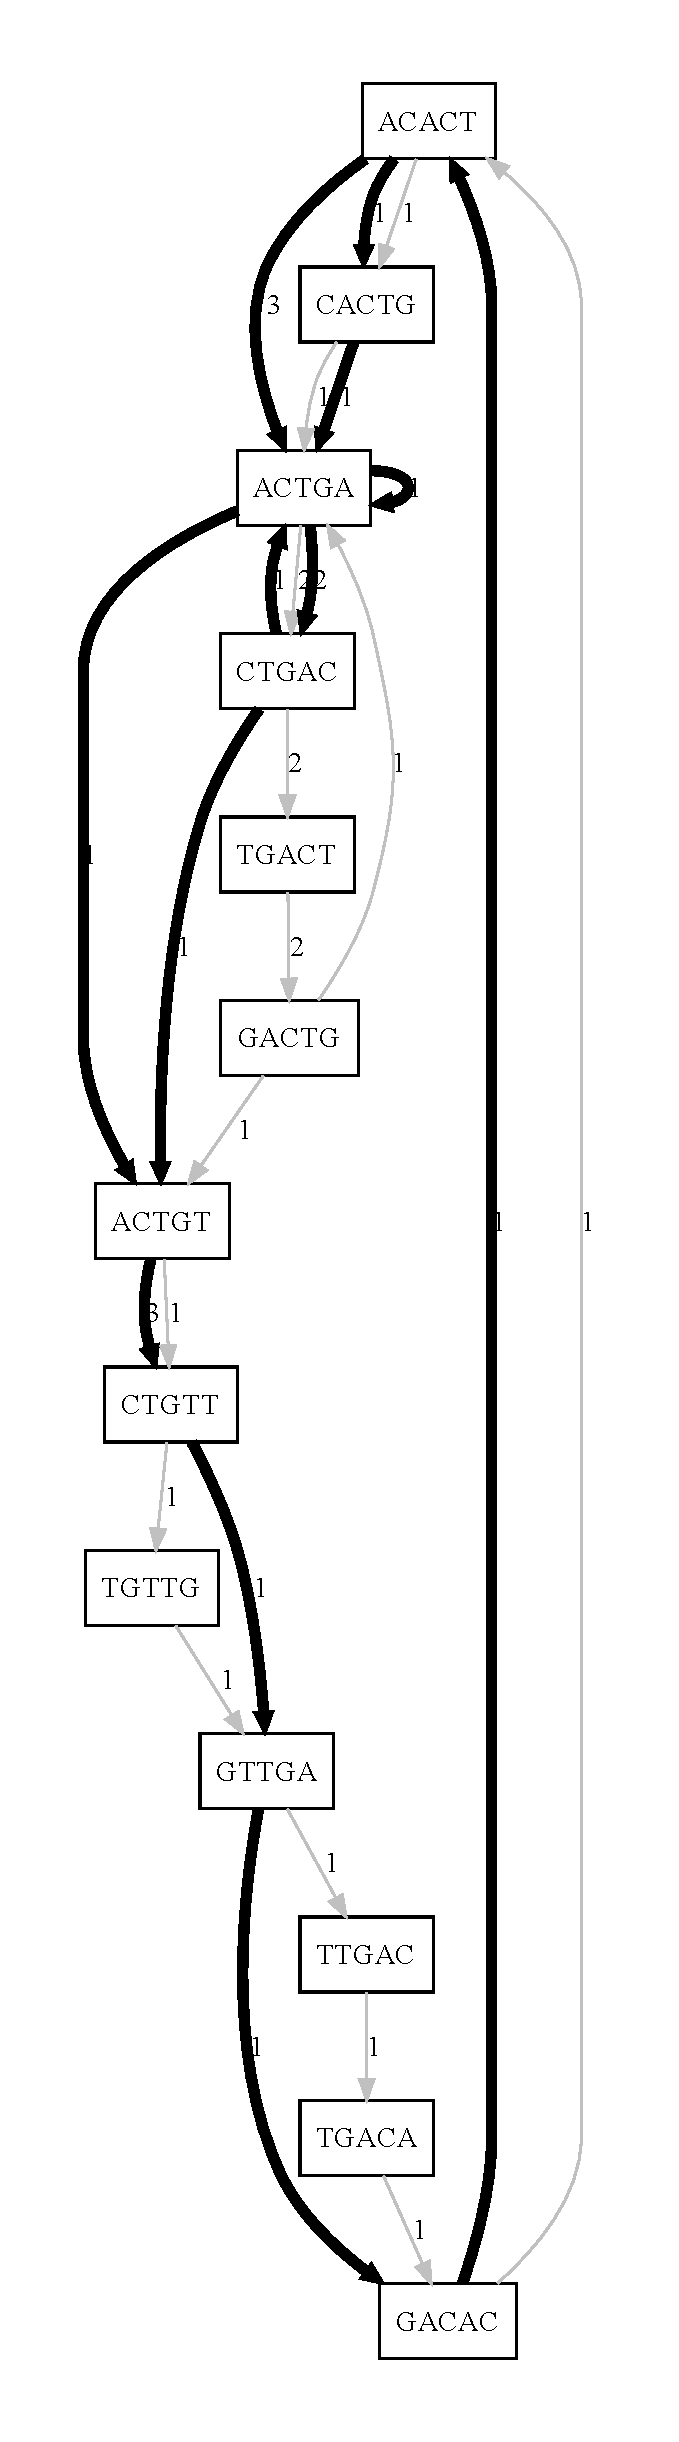
\includegraphics[height=0.9\textheight]{fig2.jpg}\end{center}
\end{figure}


The main question that still needs to be answered is:
does this graph really represent the repeat structure of the genome?

\section{Some further ideas}
\subsection{Reducing the number of vertices}
As said in the beginning the main motivation for considering such graphs
they contain fewer edges than the original de Bruijn graph. Clearly, the number of edges in
A Bruijn graph is also reduced (the vertices with no bold adjacent edges actually do not belong
to A Bruijn graph). In order to further reduce the number of vertices we one can do the following.
First, mark just one $k$-mer in each read with the minimal possible hash value. If it turned out to be
the first or the last $k$-mer of the current read, mark one more $k$-mer with the next smallest hash 
value. This guarantess that in case each possible read is present in the set of reads
at least two $k$-mers will be marked in each read. We then add edges between marked $k$-mers
that are present in the same read. In practice, not all the reads may be present and 
reads contain errors, so it makes sense to additionally check whether ta least two $k$-mers
are marked in each read.



\end{document}
